%
% Example beamer presentation using the Purdue theme with the 
% School of Aeronautics and Astronautics (AAE) banner
%
% Use pdfLatex to compile

% Use these options for printing handouts:
%\documentclass[english,handout]{beamer}
%
% Use this option for creating the presentation slides
\documentclass[english]{beamer}

\usetheme{Boadilla}
\makeatletter
\setbeamercovered{transparent}
\usecolortheme{purdue}
\usepackage{pgfpages}

% For printing handouts, uncomment the next line:
%\pgfpagesuselayout{4 on 1}[letterpaper,border shrink=0.25in,landscape]

% These are required for making the AAE banner:
\usepackage{tikz,xmpmulti}

% These are some useful packages:
\usepackage{amsmath,amssymb}
\usepackage{graphicx,geometry,lmodern}
\usefonttheme[onlymath]{serif}
\usepackage[hypcap]{caption}
\usepackage{fancyvrb,fancyref,framed}
\usepackage{subcaption}

% Short Title goes in bottom bar; Long Title is only on first slide:
\title[Short Title]{\textbf{Long Title of the\\Presentation\\with Line Breaks}}

% Short author name is in bottom left bar; long name is only on first slide:
\author[F. L-N]{First \& Last-Name}

\date{{\scriptsize April 24, 2015}}

\institute[Purdue University]
{
  School of Aeronautics \& Astronautics\\
  Purdue University
}


% User-defined commands to save time:
\newcommand{\bs}[1]{\boldsymbol{#1}} % this means \bs{} is the same as \boldsymbol{}
\newcommand{\inv}[1]{#1^{-1}}        % this means \inv{} is the same as {...}^{-1}

% Create the document:
\begin{document}

% First frame is the title slide:
\begin{frame}
% The AAE banner goes here:
\tikz [remember picture,overlay]
    \node at
    ([anchor=west,yshift=-0.23in,xshift=0]current page.north)
    {
\includegraphics[width=1.07\textwidth]{AAE_banner}};

\bigskip
\titlepage
\end{frame}

% Second frame (optional) is the table of contents:
\begin{frame}{Outline}
\tableofcontents
\end{frame}


% Sections are used to build the table of contents (optional):
%
%  %  %  %  %  %  %  %  %  %  %  %  %  %  %  %  %  %
\section{Introduction}
%  %  %  %  %  %  %  %  %  %  %  %  %  %  %  %  %  %

% Section heading slide:
\begin{frame}
\begin{center}
{\LARGE \textsc{Introduction}}
\end{center}
\end{frame}

% If you add {slide title} after {frame} it adds the title and black bar:
\begin{frame}{Introduction}
%
% Blocks are nice features:
\begin{block}{Scope}
\begin{itemize}
\item Develop ...
\item Prove ...
\item Apply ...
\end{itemize}
\end{block}
%
% The \pause command helps with lots of text
%  (you can put as many pauses as you like):
\pause
%
\begin{block}{Specific Contributions}
\begin{itemize}
\item First achievement
\item Second achievement
\item Third achievement
\end{itemize}
\end{block}
%
\end{frame}

% Subsections are also optional:
\subsection{Motivation}

\begin{frame}{Motivation}
%
% I use the figure and minipage environments to put several pictures together:
%
\begin{figure}[!hbtp]
\centering
    \begin{subfigure}[c]{0.4\textwidth}
    {\scriptsize Google drone delivery$^1$} \\
    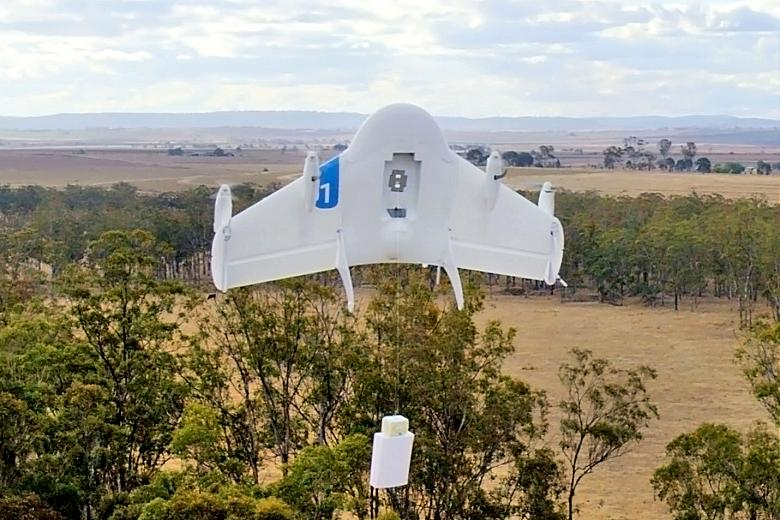
\includegraphics[width=1.5in]{pics/google_drone.jpg}
    \end{subfigure}%
$\quad$
    \begin{subfigure}[c]{0.4\textwidth}
    {\scriptsize Amazon drone delivery$^2$}\\
    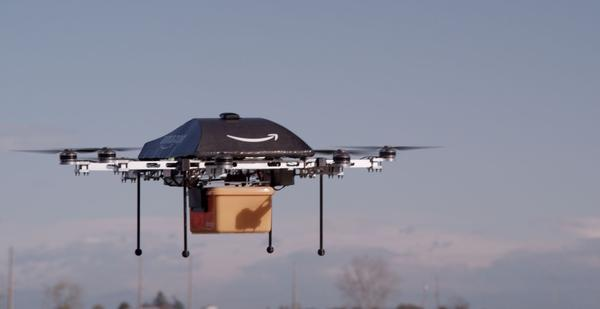
\includegraphics[width=1.8in]{pics/amazon_drone.jpg}
    \end{subfigure}
    \\ \vspace{3pt}
    \begin{subfigure}[c]{0.4\textwidth}
    {\scriptsize Bladeworx's light-rail surveillance$^3$} \\
    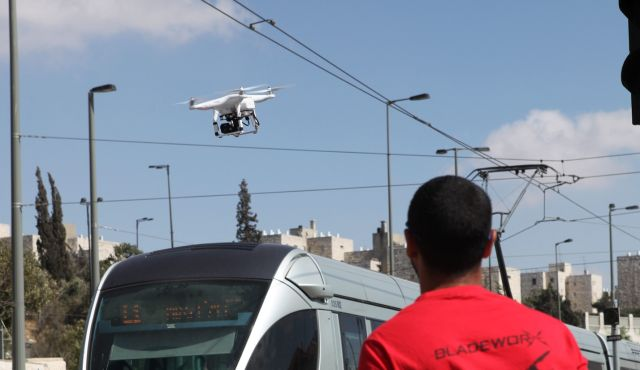
\includegraphics[width=1.5in]{pics/jerusalem_drone.jpg}
    \end{subfigure}%
$\quad$
    \begin{subfigure}[c]{0.4\textwidth}
    {\scriptsize BP pipeline inspection$^4$}\\
    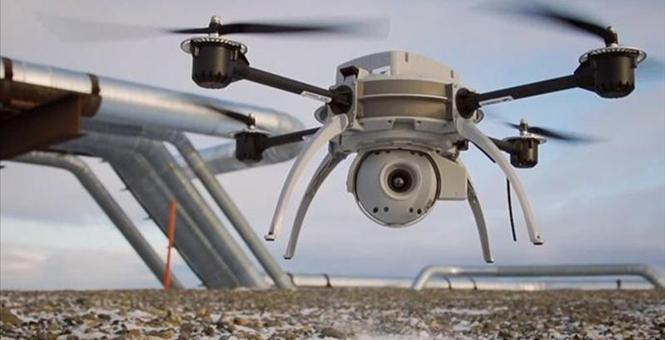
\includegraphics[width=1.8in]{pics/bp_drone.jpg}
    \end{subfigure}
    \end{figure}
\vfill
\hrulefill % this makes a horizontal line

{\tiny %
1) www.thetimes.co.uk/tto/business/industries/technology/%
article4190571.ece\\ \vspace{-1pt}
2) articles.latimes.com/2013/dec/03/business/la-fi-tn-amazon-ups-google-delivery-drones-20131203 \\ \vspace{-1pt}
3) www.smartrailworld.com/how\_drones\_are\_already-being-used-by-railways-around-the-world \\ \vspace{-1pt}
4) townhall.com/news/us/2013/06/07/in-alaskas-oilfields-drones-countdown-to-takeoff-n1615231 \\ \vspace{-1pt}
}
%
\end{frame}


\subsection{Preliminary Theory}

\begin{frame}{Preliminary Theory \& Notation}
%
Consider the uncertain nonlinear system described by
\begin{align*}
\dot{x} = \bs{\varphi}(x)^T \bs{\theta} + \Delta(x,t) + u
\end{align*}
\pause
where, \vspace{-12pt}
\begin{align*}
x \; &: \; \text{the state (scalar)} \\
\bs{\varphi}(x) \; &: \; \text{vector of known basis functions} \\
\bs{\theta} \; &: \; \text{vector of uncertain parameters} \\
\Delta(x,t) \; &: \; \text{disturbances \& unmodeled dynamics} \\
u \; &: \; \text{control input}
\end{align*} \bigskip
%
%
\pause
For example, if 
$ \quad
\dot{x} = a\, \sin x + d(x,t) + u
$
, then \vspace{-12pt}
\begin{align*}
\bs{\varphi} = \sin x \;, \quad \bs{\theta} = a \;, \quad \Delta(x,t) = d(x,t)
\end{align*}
%
\end{frame}


%  %  %  %  %  %  %  %  %  %  %  %  %  %  %  %  %  %
\section{Conclusion}
%  %  %  %  %  %  %  %  %  %  %  %  %  %  %  %  %  %

\begin{frame}{Conclusion}
%
Journal Papers:
\begin{small}
\begin{itemize}
\item Submitted journal paper number 1
\item Submitted journal paper number 2
\end{itemize}
\end{small}
%
\end{frame}


%  %  %  %  %  %  %  %  %  %  %  %  %  %  %  %  %  %
\section{Appendix}
%  %  %  %  %  %  %  %  %  %  %  %  %  %  %  %  %  %

\begin{frame}
\begin{center}
{\LARGE \textsc{Appendix: \\Supporting Materials}}
\end{center}
\end{frame}

\begin{frame}{Projection-based Adaptation} \label{eqn:proj-def}
The discontinuous projection is defined as follows.
%
%
\begin{align}
\text{Proj}_{\hat{\theta}_i}(\bullet_i) := \begin{cases}
0 & \text{if } \; \begin{cases} 
\hat{\theta}_{i} = \hat{\theta}_{i,max} \; \text{ and } \; \bullet_i>0 \\
\hat{\theta}_{i} = \hat{\theta}_{i,min} \; \text{ and } \; \bullet_i<0 
\end{cases} \\
\bullet_i \qquad &\text{otherwise}
\end{cases} \nonumber
\end{align}

This guarantees that $\hat{\bs{\theta}}(t) \in \Omega_\theta$ for all $t$, and therefore $\tilde{\bs{\theta}}(t)$ is bounded.

\end{frame}


\end{document}